\Chapter{Reactor Antineutrinos}
\label{Ch2}

    Neutrinos can be categorized by the sources they are generated from, including natural sources and artificial sources.
    The solar neutrino, relic neutrino, supernova neutrino, geo-neutrino, and atmospheric neutrino are neutrinos generated by natural cosmological or radioactive sources.
    Reactor antineutrinos (henceforth mentioned as \textit{reactor neutrinos}) and accelerator neutrinos are human-made.
    
    Reactor neutrino experiments have the advantages of
    \begin{itemize}
        \item Relatively high statistics;
        \item Easy-to-control experimental baselines;
        \item A relatively narrow range of neutrino energy.
    \end{itemize}
    Thus, reactor neutrino experiments have played an irreplaceable role in the history of neutrino detection and oscillation measurements.
    
\Section{The Flux and Spectrum of Reactor Neutrinos}
    
    Reactor neutrinos are \nuebar generated through $\beta$-decay of the daughter nuclei of the nuclear fission process.
    Since the discoveries of lepton number conservation and neutrino flavors, Equation~\ref{eq1.1} is rewritten as the decay of a neutron producing \nuebar,
    \begin{equation}\label{eq2.1}
        n \rightarrow p + e^- + \nuebar,
    \end{equation}
    where the proton is contained in a daughter nucleus.
    The chain reaction of a nuclear reactor produces a great variety of fission produced isotopes that release their energy through beta decay.
    One fission reaction naturally results in the emission of multiple neutrinos, most with kinetic energy ranging from  0~MeV to 10~MeV.
    
   	Fission reactions of most reactor cores are dominated by \Ulow , with other fission isotopes including $^{238}$U, $^{239}$Pu and $^{241}$Pu.
    The spectrum of reactor neutrinos is expressed as
    \begin{equation}\label{eq2.2}
        S(E_\nu) = \frac{W_{reactor}}{\sum_i \frac{f_i}{F}e_i}\sum_i\frac{f_i}{F}(\frac{dN_i}{dE_\nu}),
    \end{equation}
    where $W_{reactor}$ is the thermal power of the reactor, $i$ is each of the four fission isotopes above, $f_i/F$ is the relative fraction of each isotope, $e_i$ is energy per fission, and 
    \begin{equation}
        \frac{dN_i}{dE_\nu} = \sum_n Y_n(t)(\sum_j b_{n,j}\cdot P(E_\nu, E_0^{n,j})),
        \label{eq:23}
    \end{equation}
    which is the summed energy spectrum of each fission isotope.
    In Equation~\ref{eq:23}, $Y_n(t)$ is cumulative fission yield, $b_{n,j}$ are the $\beta$-branches, and $P(E_\nu, E_0^{n,j})$ is the spectrum of each branch.
    A typical reactor has thousands of $\beta$-decay branches. 
    By adding the neutrino spectra of these branches, one can predict the spectrum of neutrinos generated from a reactor, an illustration is shown in Figure~\ref{fig:2.1}.
    \begin{figure}[h!]\label{fig:2.1}
    \centering
    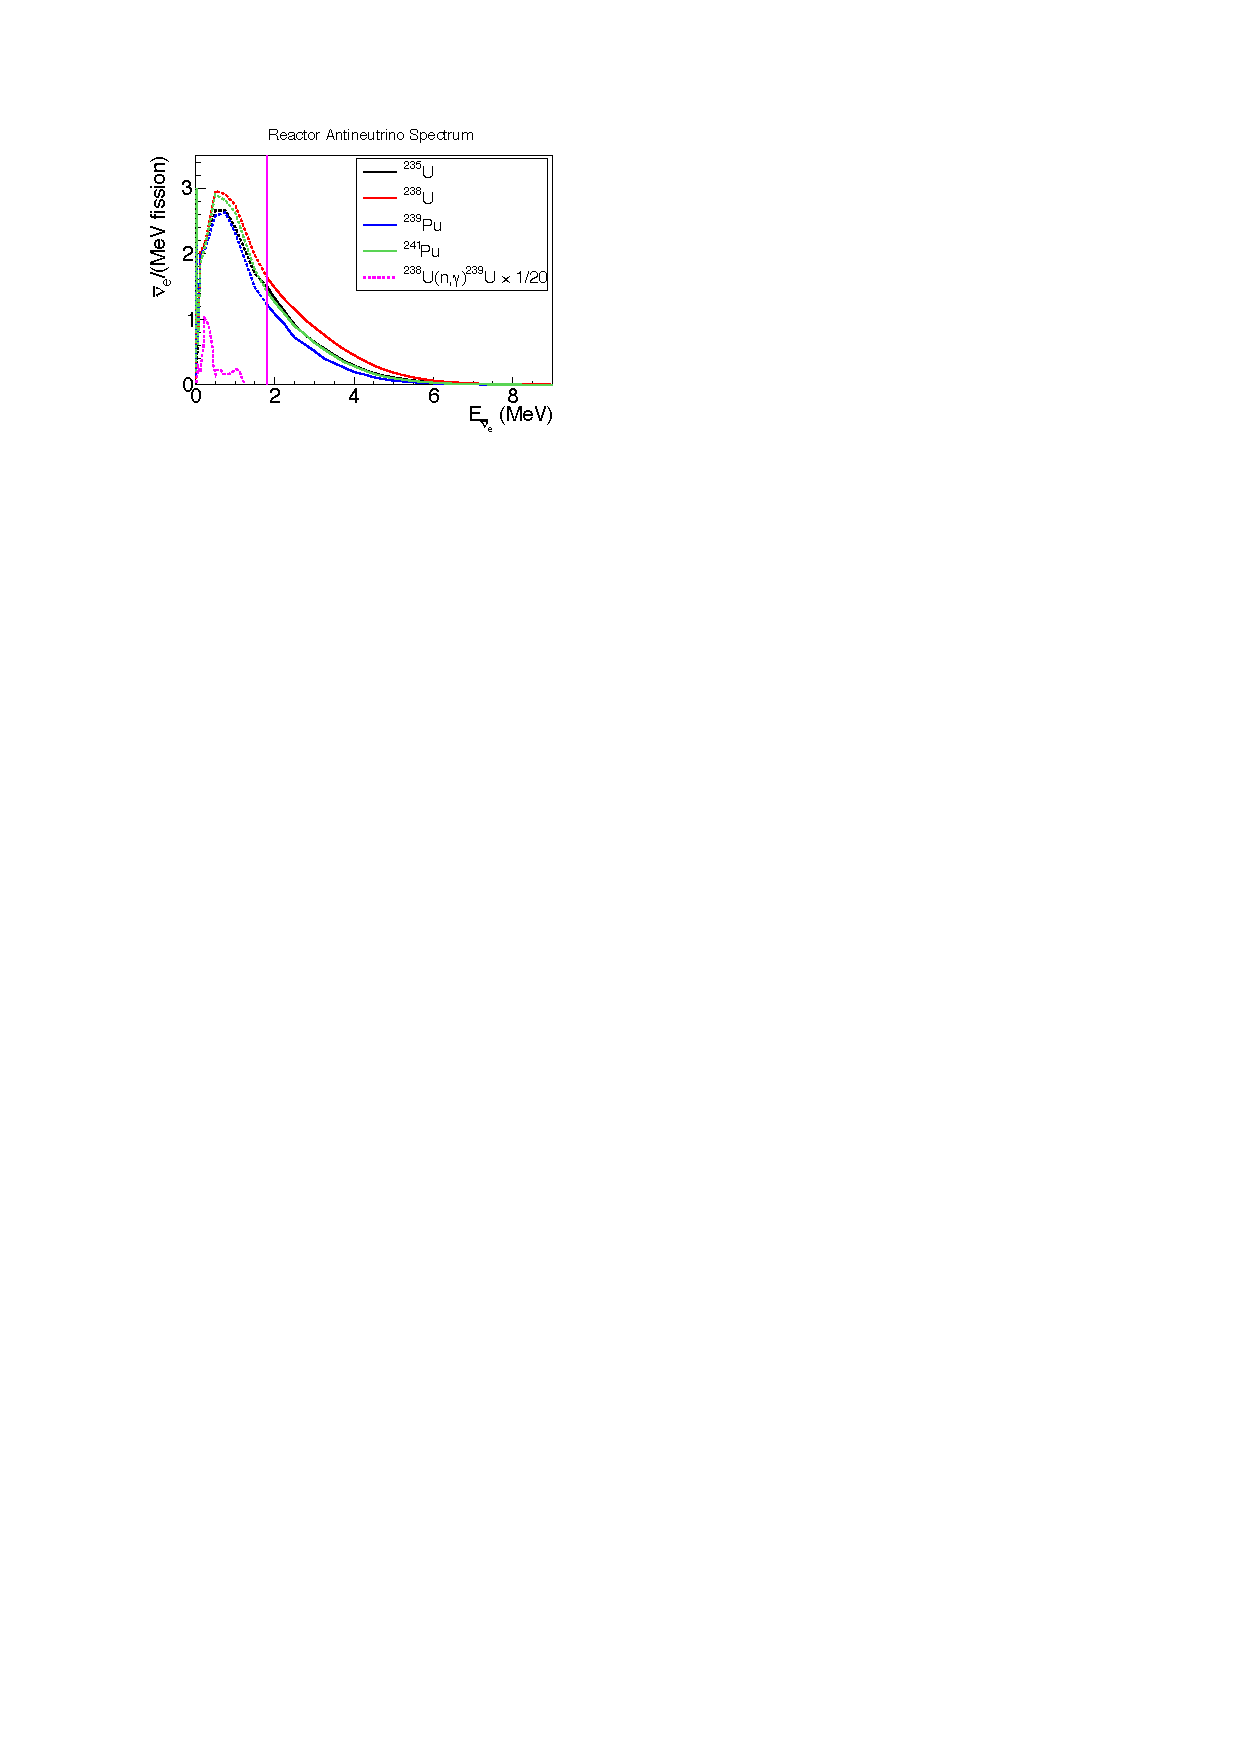
\includegraphics[width=0.6\textwidth]{Figures/RxNeutrinoSpec.pdf}
    \caption[Predicted reactor neutrino spectrum]{An illustration of a commercial reactor neutrino spectrum prediction~\cite{bib:Qian2019}.}
    \end{figure}  

    Reactor neutrino experiments rely on the detection of the IBD process expressed in Equation~\ref{eq1.1}.
    Because of the mass difference between the neutron and proton, the neutrino energy $E_\nu$ must be above a threshold to trigger the IBD process, as
    \begin{equation}\label{eq2.4}
    E_\nu \ge m_n + m_e - m_p \simeq 1.806 \textrm{MeV}.
    \end{equation}
    The kinectic energy of the IBD produced neutron $T_n$ is on the keV scale.
    Thus, the total energy of an IBD positron can be expressed as
    \begin{equation}\label{eq2.5}
    E_e = E_\nu - (m_n + T_n - m_p) \simeq E_\nu - 1.293 MeV.
    \end{equation}
    In an IBD detector, the $e^+$ quickly annihilates with an atomic electron and emits two 0.511~MeV $\gamma$ rays.
    The visible energy of an IBD positron in an ideal detector is 
    \begin{equation}\label{eq2.6}
    E_{vis} \simeq E_\nu - 0.782 MeV,
    \end{equation}
    which is a useful direct experimental conversion for the reconstruction of the \nuebar energy. 
    The cross-section of the IBD interaction is dependent on the neutrino energy and can be expressed as a function of positron energy
    \begin{equation}\label{eq2.7}
    \sigma_{IBD} \simeq \frac{2\pi^2}{\tau_n m_e^5 f }E_eP_e = 10^{-43}\cdot \frac{E_ep_e}{\textrm{MeV}}\cdot(\frac{\tau_n}{886\textrm{s}})^{-1} \textrm{cm}^2,
    \end{equation} 
    where $\tau_n$ is the neutron lifetime and $f$ is a phase space integral factor.
    Based on the theoretical neutrino spectrum (Equation~\ref{eq2.2}) and IBD cross-section (Equation~\ref{eq2.7}), a reactor neutrino experiment can expect a measured spectrum and flux as shown in Figure~\ref{fig:2.2}.
    \begin{figure}[h!]
    \centering
    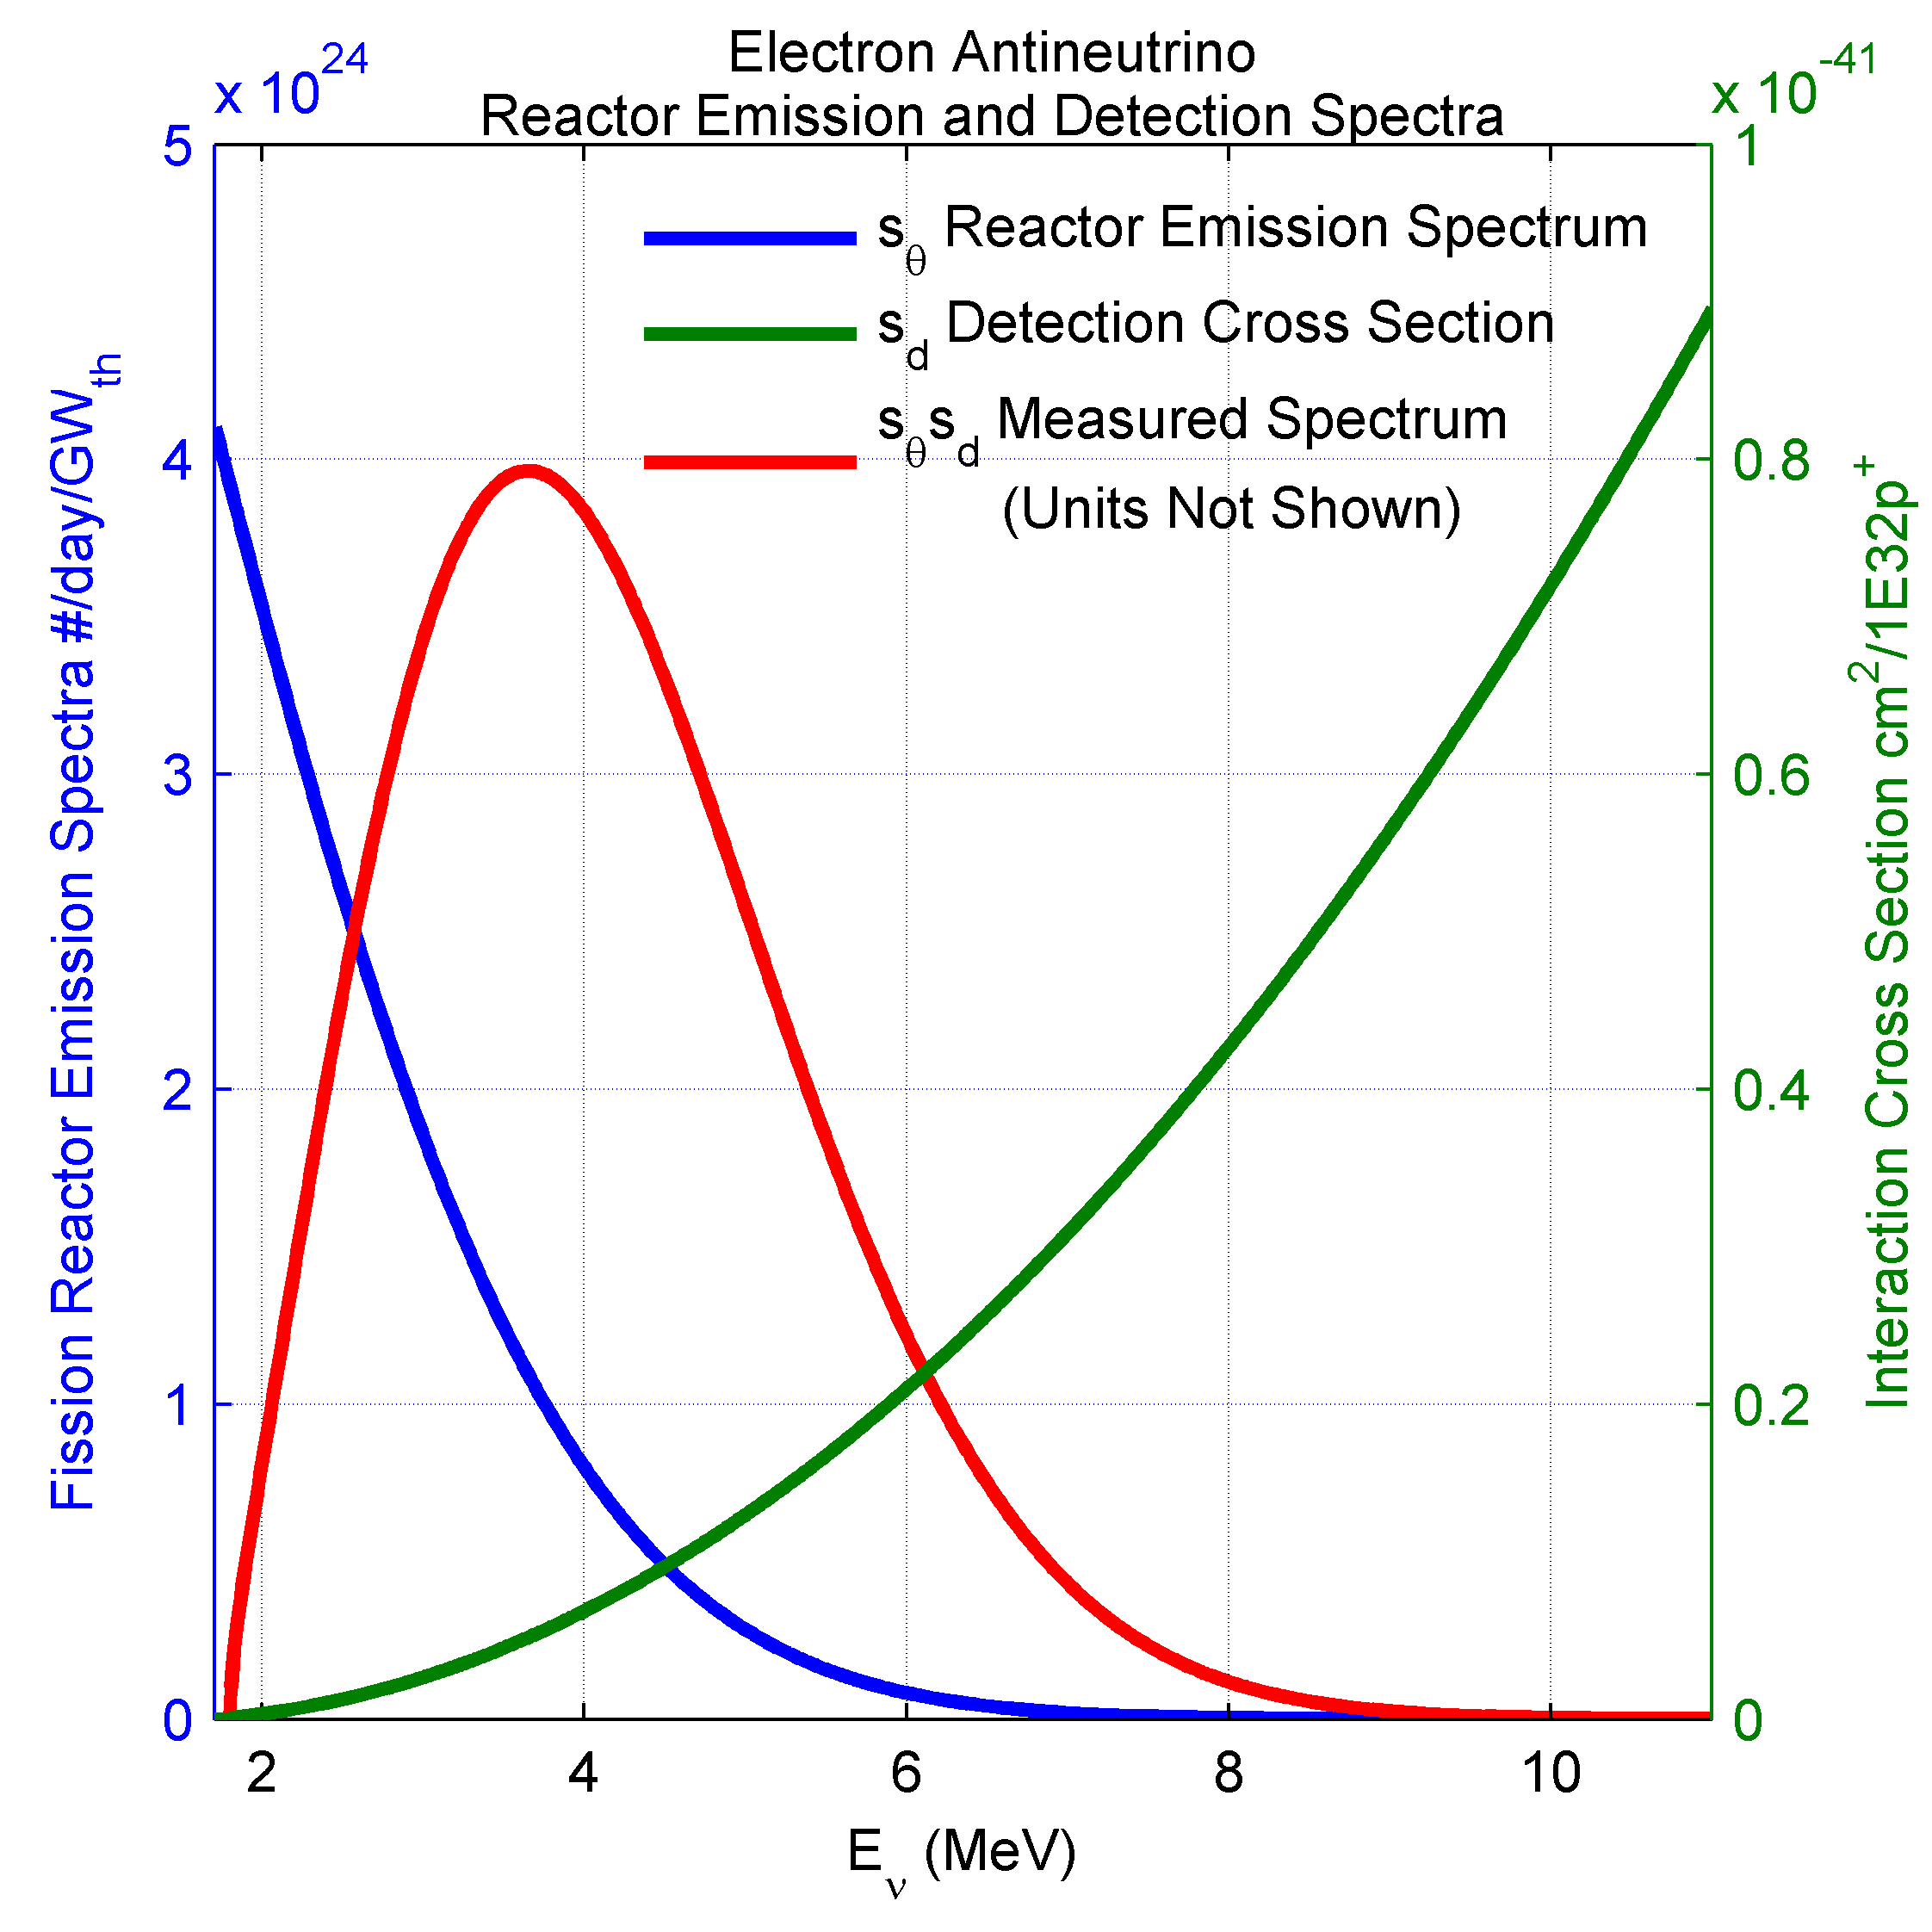
\includegraphics[width=0.6\textwidth]{Figures/twoXsections.png}
    \caption[Expectation of detected reactor neutrino spectrum]{An illustration~\cite{bib:Jocher} of the detected neutrino energy spectrum in a reactor experiment. 
    The detected spectrum is the multiplication of the emitted neutrino spectrum and IBD cross-section.}
    \label{fig:2.2}
    \end{figure}      
    
    Reactor neutrino research has an interest in testing the success of nuclear and particle physics theories by comparing experimental measurements of reactor neutrino flux and spectra to predictions based on these theories.
    There are two methods to predict the absolute neutrino spectrum of a nuclear reactor:
    \begin{itemize}
        \item \textbf{The \textit{ab initio} method:} The neutrino spectrum is calculated by Equation~\ref{eq2.2} and \ref{eq:23},
        where the ratio and the endpoint energy of each branch are extracted from data in nuclear databases, such as Evaluated Nuclear Structure Data File (ENSDF)~\cite{bib:ENSDF}, ENDF~\cite{bib:ENDF}, and Japanese Evaluated Nuclear Data Library (JENDL)~\cite{bib:JENDL}.
        The predicted neutrino spectrum is the sum of the calculated $\beta$-spectra including a variety of theoretical corrections. 
        The most-widely used neutrino spectrum of $^{238}$U is predicted in this way~\cite{bib:vogel}.
        \item \textbf{$\beta$-conversion method:} Because the kinetic energy of the $\beta$-decay proton is negligibly small, the total $\beta$-decay end point energy $E_0 \simeq E_\nu + E_e$.
        The neutrino spectrum can thus be deduced from the experimental measurement of $\beta$ energy from a fission reactor. 
        In the 1980s, the $^{235}$U, $^{239}$Pu, and $^{241}$Pu neutrino spectra were converted from the spectrum measurements of $\beta$s from the Institut Laue-Langevin (ILL) reactor~\cite{bib:ILL1982,bib:ILL1985,bib:ILL1989}.
        The conversion was made by fitting the measured $\beta$ spectrum with the sum of tens of hypothetical $\beta$-decay branches, then converting the spectrum of each $\beta$ branch to a neutrino spectrum.
    \end{itemize}
    The detailed theoretical approaches are described in Section 2.3.
    
    Successful neutrino flux and spectrum prediction and measurement made it possible for reactor neutrino experiments to test the nuclear model of fission reactors.

\Section{Historical Context of Reactor Neutrino Experiments}

    After the discovery of neutrinos via the detection by the Savannah reactor neutrino experiment~\cite{bib:CowanReines}, a hint of $\nuebar$ oscillation was discovered by Reines \textit{et al} in 1980~\cite{bib:reines1980}.
    Their experiment found in unexpected ratio between CC and NC interactions at the $2\sigma-3\sigma$ level of statistical significance, which suggests antineutrino oscillation.
    More reactor experiments were built to test \nuebar oscillation over a wide variety of baseline by comparing neutrino flux to theoretical predictions or to measurements at different baselines, included in Table~\ref{tab:history}.
    These experiments attempted to observe neutrino oscillation via \nuebar  disappearance.
    The commonly used methods are to compare the observed neutrino flux to the expected flux, or to compare the relative flux/spectrum difference at different baselines.
    \begin{table}[!htbp]
    \centering
    \caption[An overview of historical reactor oscillation experiments]{An overview of historical reactor experiments searching for \nuebar oscillation in baseline from $\sim$10~m to $\sim$100~km.
    The absolute flux ratios were calculated by comparing experimental measurements to the expected fluxes.
    The relative flux indicates the ratio of neutrino flux measured by detectors at different baselines.}
    \begin{tabular}{lllll}
    \hline
    \hline
    Experiment  & Baseline   & Absolute flux  & Relative flux    & Reference   \\ 
    \hline
    ILL     & 8.76~m  & $0.955\pm 0.115$  &  & \cite{bib:kwon1981}  \\
    \hline
        & 37.9~m   & $1.018\pm 0.06$  &   &   \\
    G\"osgen  & 45.9~m  & $1.045\pm 0.06$  &   & \cite{bib:gosgen}  \\
        & 64.7~m    & $0.975\pm 0.06$  &   &   \\
    \hline
    Rovno     & 18.3~m to 25.3~m     & $0.964\pm 0.068$  &   & \cite{bib:Afonin1987}  \\
    \hline
    Krasnoyarsk     &  57~m to 231~m    & $0.99\pm 0.05$  & $0.86\pm 0.15$  &  \cite{bib:Vidyakin1994} \\
    \hline
        & 14~m & $0.988\pm 0.05$  &   &   \\
    Bugey   & 40~m  & $0.994\pm 0.05$  &   &  \cite{bib:Bugey} \\
        & 95~m  & $0.913\pm 0.13$  &   &   \\
    \hline
    Savannah River  &  18~m & $0.987\pm 0.038$ &    & \cite{bib:Greenwood1996} \\
        &4~m    & $1.055\pm 0.038$  &   &   \\
    \hline
    CHOOZ   & 1~km     & $1.01\pm 0.04$   &   & \cite{bib:chooz98, bib:Chooz99, bib:chooz03}  \\
    \hline
    Palo Verde   &  750~m to 890~m & $1.04\pm 0.09$ &   &  \cite{bib:palo01, bib:palo1999, bib:palo2000} \\
    \hline
    KamLAND & 80~km to 800~km  &  $0.658\pm 0.06$ &   & \cite{bib:KamLAND03, bib:kamland04}  \\
    \hline
    \end{tabular}
    \label{tab:history}
    \end{table}
 
    The experiments listed in Table~\ref{tab:history} cover different regions in the $(\Delta m^2, \sin^2\theta)$ parameter space of neutrino oscillations.
    The CHOOZ and Palo Verde experiments narrowed the allowed range of the parameter space to $\sin^2 2\theta_{13} \le 0.18$ for $|\Delta m^2_{13}|\ge 2\times 10^{-3}$ eV$^2$, these results indicated that $\nu_\mu \rightarrow \nu_e$ oscillation provided only a small contribution to the atmospheric neutrino anomaly.
    
    In 2002, the KamLAND experiment~\cite{bib:KamLAND03, bib:kamland04} confirmed reactor neutrino oscillation via a spectrum measurement of \nuebar from 53 reactors around Japan (also 5\% in South Korea and 1\% from other reactors), with 180~km average baseline.
    The KamLAND experiment utilized a spherical detector with filled about 3000~ton of LS deployed in the Kamioka mine in Japan. 
    The IBD positron and neutron signals were collected by 1879 inward-facing photomultiplier tubes (PMTs) on the surface of the detector. 
    Similar to the Cowan-Reines experiment~\cite{bib:CowanReines}, KamLAND used positron-neutron time coincidence to tag the IBD interaction candidates, with the prompt positron signal followed by a delayed $\gamma$ signal from $n$-H capture in the detector.
    With 162 ton$\cdot$yr exposure, the KamLAND experiment observed neutrino oscillation at very long baselines by comparing the detected neutrino flux to the neutrino flux predicted by the ILL+Vogel model~\cite{bib:ILL1982, bib:ILL1985, bib:ILL1989, bib:vogel} shown in Figure~\ref{fig:kamFlux}.
    KamLAND also observed oscillation behavior dependent on the experimental $L/E$ ratio, as shown in Figure~\ref{fig:kamLE}.
    
    \begin{figure}[h!]
    \centering
    \subfigure[]{\label{fig:kamFlux}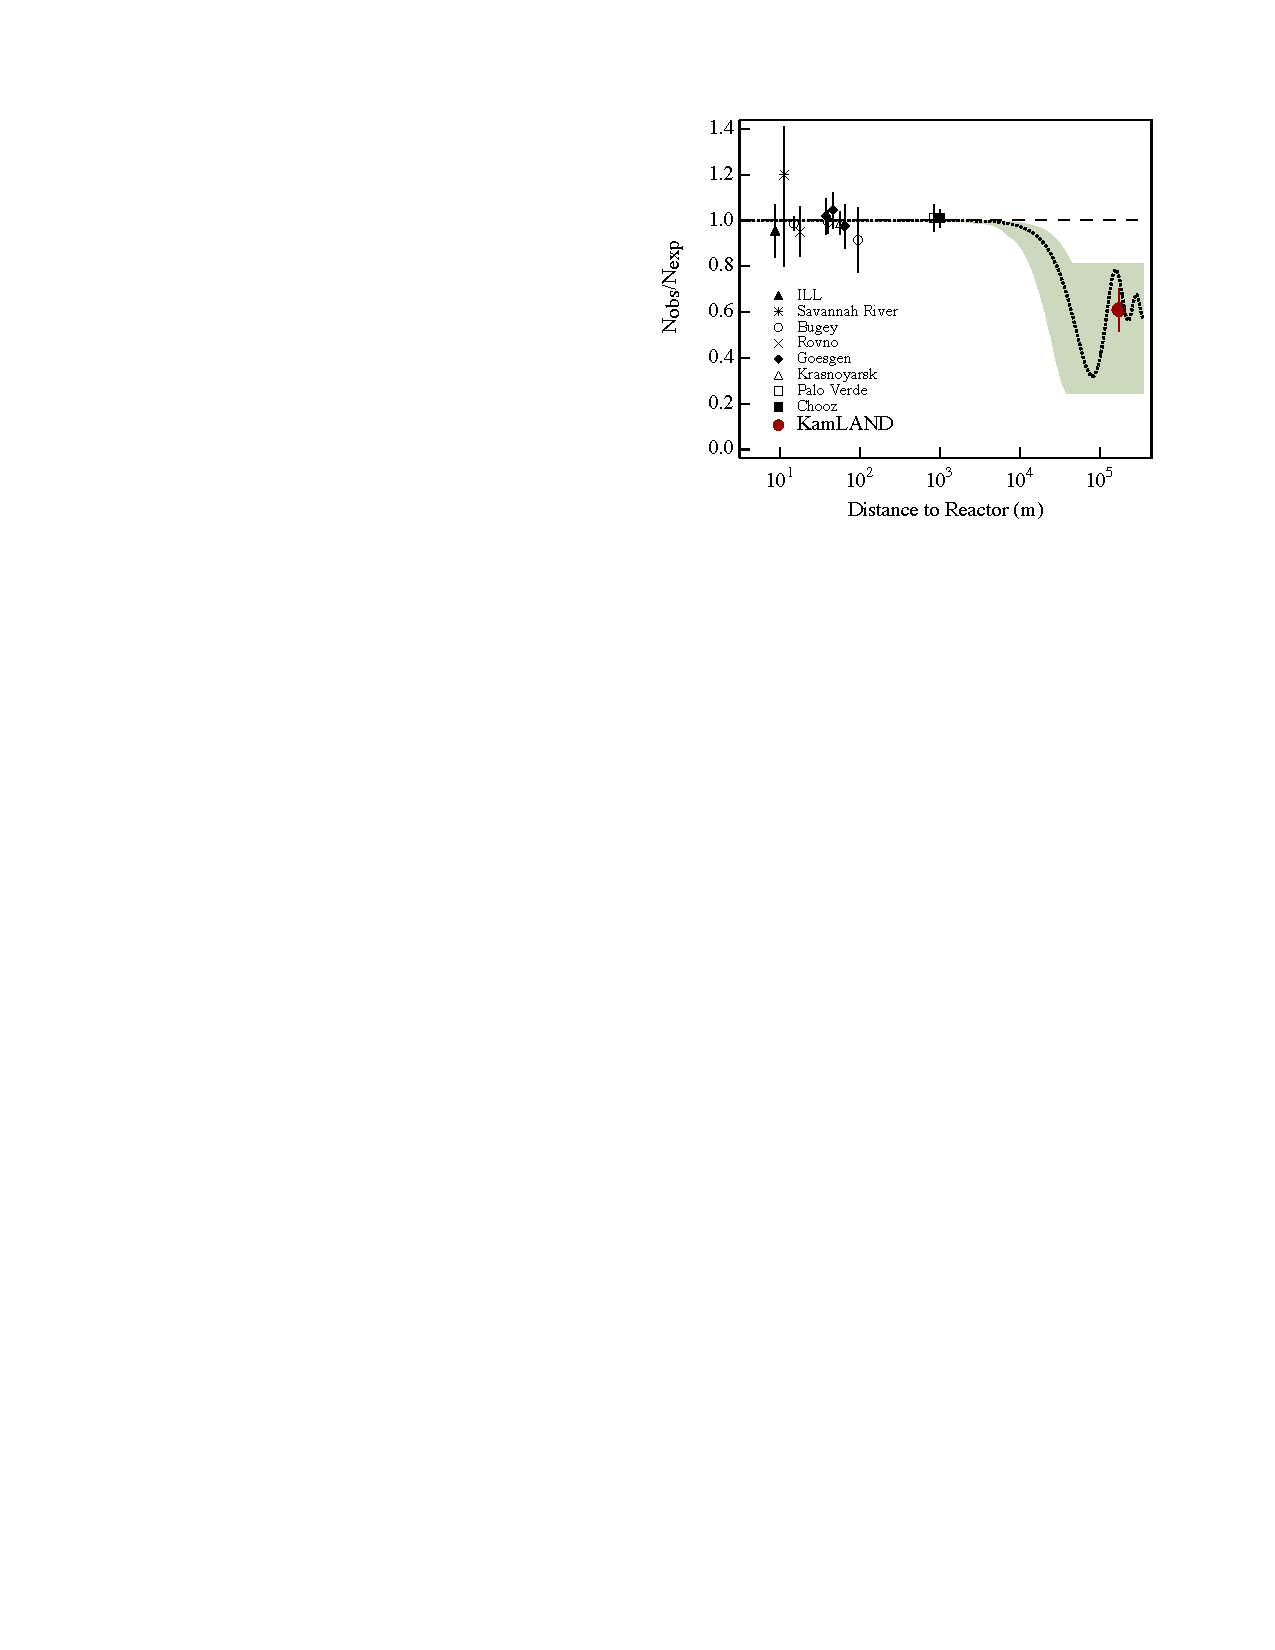
\includegraphics[width=0.48\textwidth]{Figures/KamLANDFlux.pdf}}
    \subfigure[]{\label{fig:kamLE}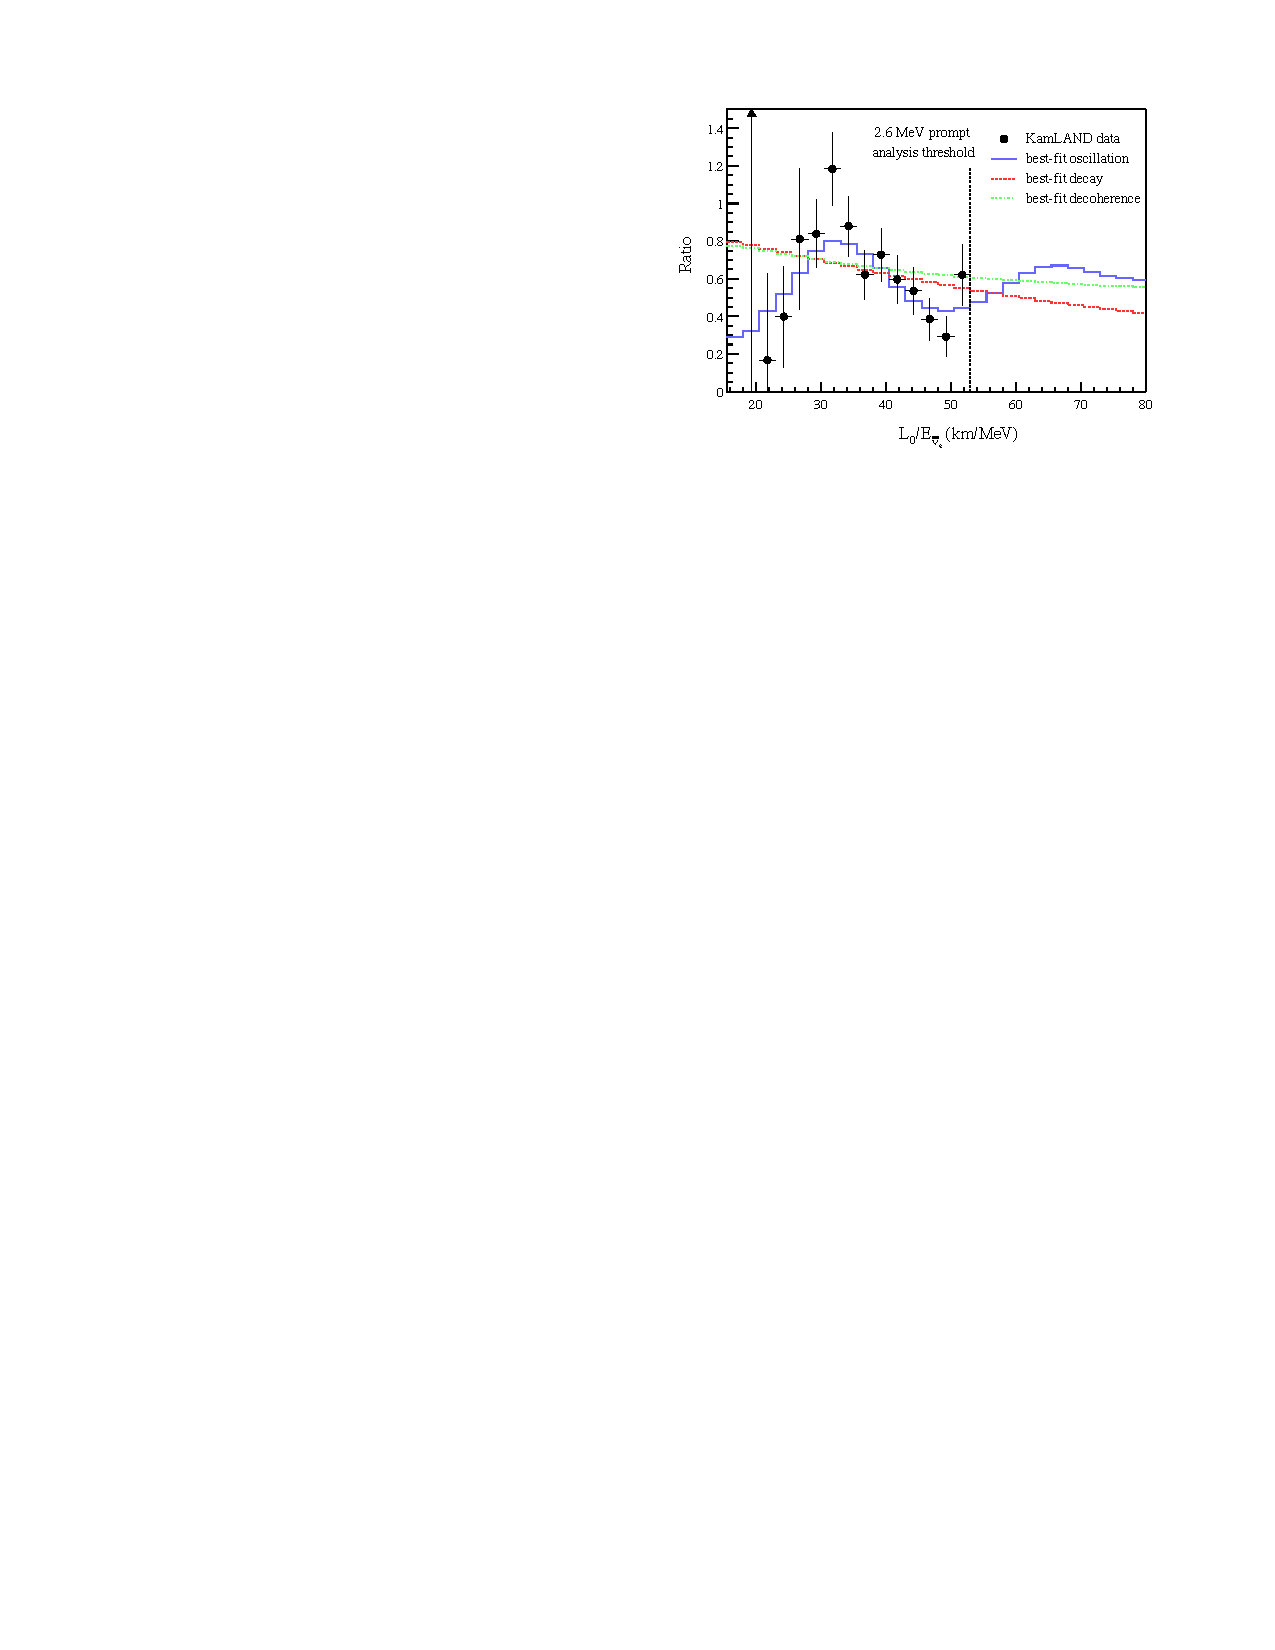
\includegraphics[width=0.48\textwidth]{Figures/KamLANDLE.pdf}}
    \caption[Confirmation of Reactor Neutrino Oscillation by KamLAND]{Observation of reactor neutrino oscillation by KamLAND~\cite{bib:kamland04}.
    (a) The ratio of the KamLAND observed neutrino flux to ILL+Vogel prediction.
    (b) The ratio of KamLAND measured $L_0/E$ spectrum to the no oscillation prediction with average baseline $L_0 = 180$~km, indicating oscillation behavior with respect to $L_0/E$ of \nuebar.
    This result also disfavored neutron decay and neutrino decoherence models made based on atmosphere neutrino experiments.}
    \label{fig:Kamland}
    \end{figure}
    
    Another milestone in reactor neutrino experiments is the precise measurement of the $\theta_{13}$ mixing angle. 
    The medium baseline experiments, CHOOZ~\cite{bib:chooz03}, Parlo Verde~\cite{bib:palo2000}, RENO~\cite{bib:RENO}, Daya Bay~\cite{bib:DYBosc} and Double CHOOZ~\cite{bib:DBChooz} attempted to measure $\theta_{13}$ via observation of $\nuebar\rightarrow\overline{\nu}$ disappearance in baselines varying from several hundred meters to 1~km from commercial reactors.
    Following CHOOZ and Parlo Verde's measurement of the $\sin^22\theta_{13}$ upper bound, RENO, Daya Bay and Double CHOOZ independently reported the measurement of a nonzero $\theta_{13}$ mixing angle.
    The three $\theta_{13}$ experiments all utilized Gd loaded LS detectors deployed at different baselines from groups of reactors.
    By comparing the \nuebar flux between near and far detectors, these experiments measured the $\nuebar\rightarrow\overline{\nu}$ disappearance probability independently from the nuclear model of the reactor \nuebar production.
    The result of the measurements are listed in Table~\ref{tab:1.1}.
    The commercial reactors utilized in these experiments contain low-enriched Uranium (LEU) fuel, whose fission isotope fractions and \nuebar productions evolve with time.
    \begin{table}[h]
    \centering
    \caption[$\theta_{13}$ reactor experiments]{Overview of results from medium baseline reactor neutrino experiments that measured the $\theta_{13}$ mixing angle~\cite{bib:RENO, bib:DYBosc, bib:DBChooz}.
}
    \begin{tabular}{ccc}
    \hline
    \hline
    Experiment  & Baseline   & Average Fission Fraction   \\ 
    \hline
    Daya Bay     & 560~m to 1640~m  & 57.1\% $^{235}$U, 29.9\% $^{239}$Pu, 7.6\% $^{238}$U, 5.4\% $^{241}$Pu \\
    RENO     & 294~m to 1383~m & 57.3\% $^{235}$U, 29.9\% $^{239}$Pu, 7.3\% $^{238}$U, 5.5\% $^{241}$Pu \\
    Double CHOOZ    & 1050~m & 48.8\% $^{235}$U, 35.9\% $^{239}$Pu, 8.7\% $^{238}$U, 6.7\% $^{241}$Pu \\
    \hline
    \end{tabular}
    \label{tab:theta13}
    \end{table}

\Section{Reactor Antineutrino Anomaly}
\label{c2s3}
        
    In addition to oscillation measurements, the $\theta_{13}$ experiments also measured the absolute neutrino flux and spectrum of the commercial reactors. 
    To provide precise models for these measurements, predictions of reactor neutrino flux and spectrum were revisited with both the \textit{ab initio} method and the $\beta$ conversion method.
    
    The `Mueller' hybrid model~\cite{bib:mueller} first used to the $\textit{ab initio}$ method by reading the ENSDF and JENDL nuclear databases to sum the \nuebar spectrum from well measured $\beta$ branches.
    This method then subtracted this summed $\beta$ spectrum from the ILL measured spectrum.
    The remaining spectra were fitted with five effective branches similar to the $\beta$ conversion method.
    This resulted in a calculated \nuebar spectra for $^{235}$U, $^{238}$U, $^{239}$Pu, and $^{241}$Pu, with limited effects from hypothetical branches.
    The `Huber' model~\cite{bib:huber} purely utilized the $\beta$ spectra of $^{235}$U, $^{239}$Pu, and $^{241}$Pu measured from the ILL reactor and applied the conversion method with higher-order theoretical corrections to the $\beta$ spectra of the virtual decay branches.
    The theoretical corrections include the effect of electron-nucleus interactions, radiation effects, and weak magnetism corrections. 
    With different approaches predicting the \nuebar spectrum, the Mueller model of expected neutrino flux found 2.5\% more than the ILL+Vogel model, and Huber model found a 3\% increase in the neutrino flux prediction.
    However, the absolute flux measurements of the historical reactor experiments within 1~km baseline showed inconsistent measured neutrino flux with respect to either of the two predictions, as shown in Figure~\ref{fig:DYBFlux}.
    \begin{figure}[h!]
    \centering
    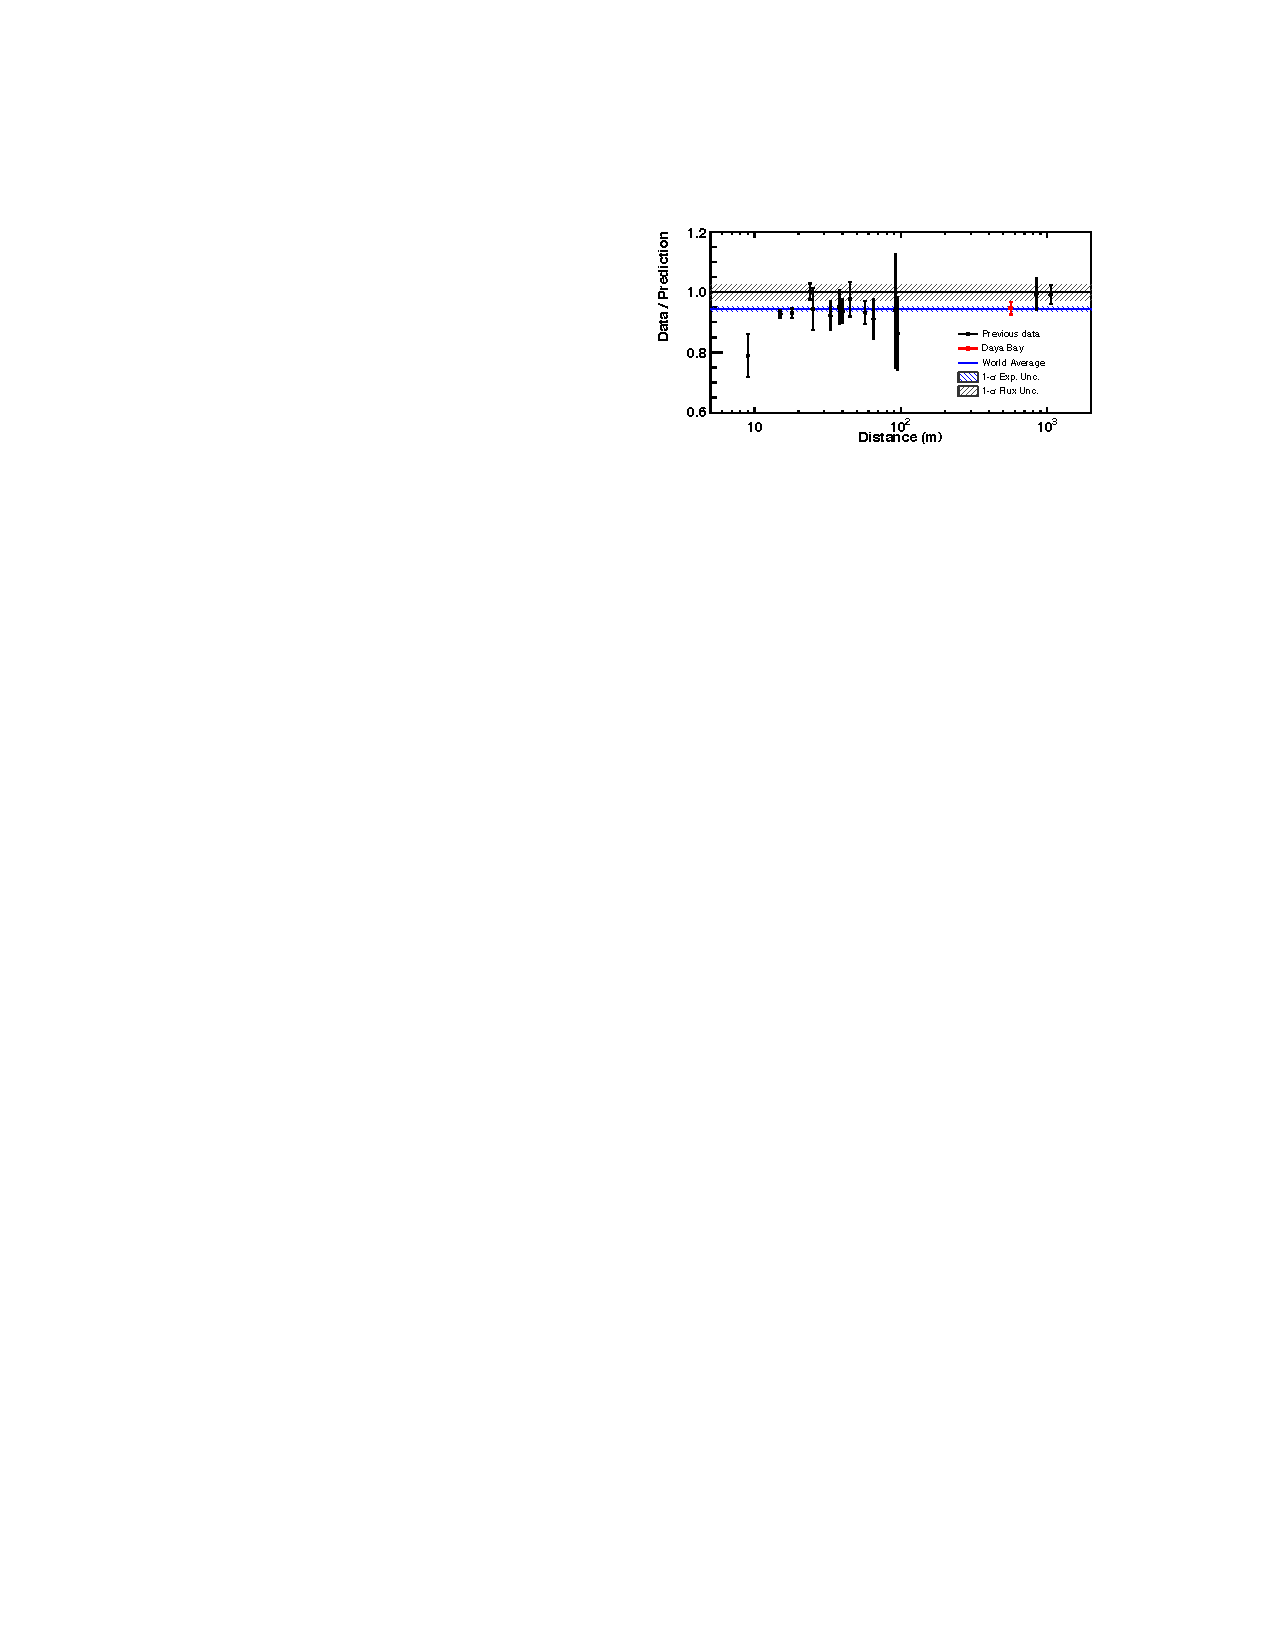
\includegraphics[width=0.8\textwidth]{Figures/DYBGlobalFlux.pdf}
    \caption[Historical Absolute Reactor Neutrino Flux]{Historical reactor neutrino flux measurements \cite{bib:DYB2015}.
    The global average is a 5\% to 6\% deficit from Huber+Mueller predicted flux.}
    \label{fig:DYBFlux}
    \end{figure}
    
    This measured neutrino flux deviation is referred to as the Reactor Antineutrino Anomaly (RAA)~\cite{bib:RAA}.
    This anomaly suggests a systematic bias present in the theoretical aggregation method and/or the virtual branching approach in the conversion from the ILL measured $\beta$ spectrum.
    This disagreement of neutrino flux in the medium baselines can also be explained by a possible oscillation between \nuebar and a light sterile neutrino.
    A 3+1 model of left-handed neutrino mixing with a sterile neutrino with $\Delta m^2\sim$1~eV$^2$~\cite{bib:RAA, bib:whitepaper} scale was developed based on the disappearance rate shown in the flux deficit.
    The RAA best fit 3+1 neutrino oscillation parameters are shown in Figure~\ref{fig:RAA}.
\begin{figure}[h!]
    \centering
    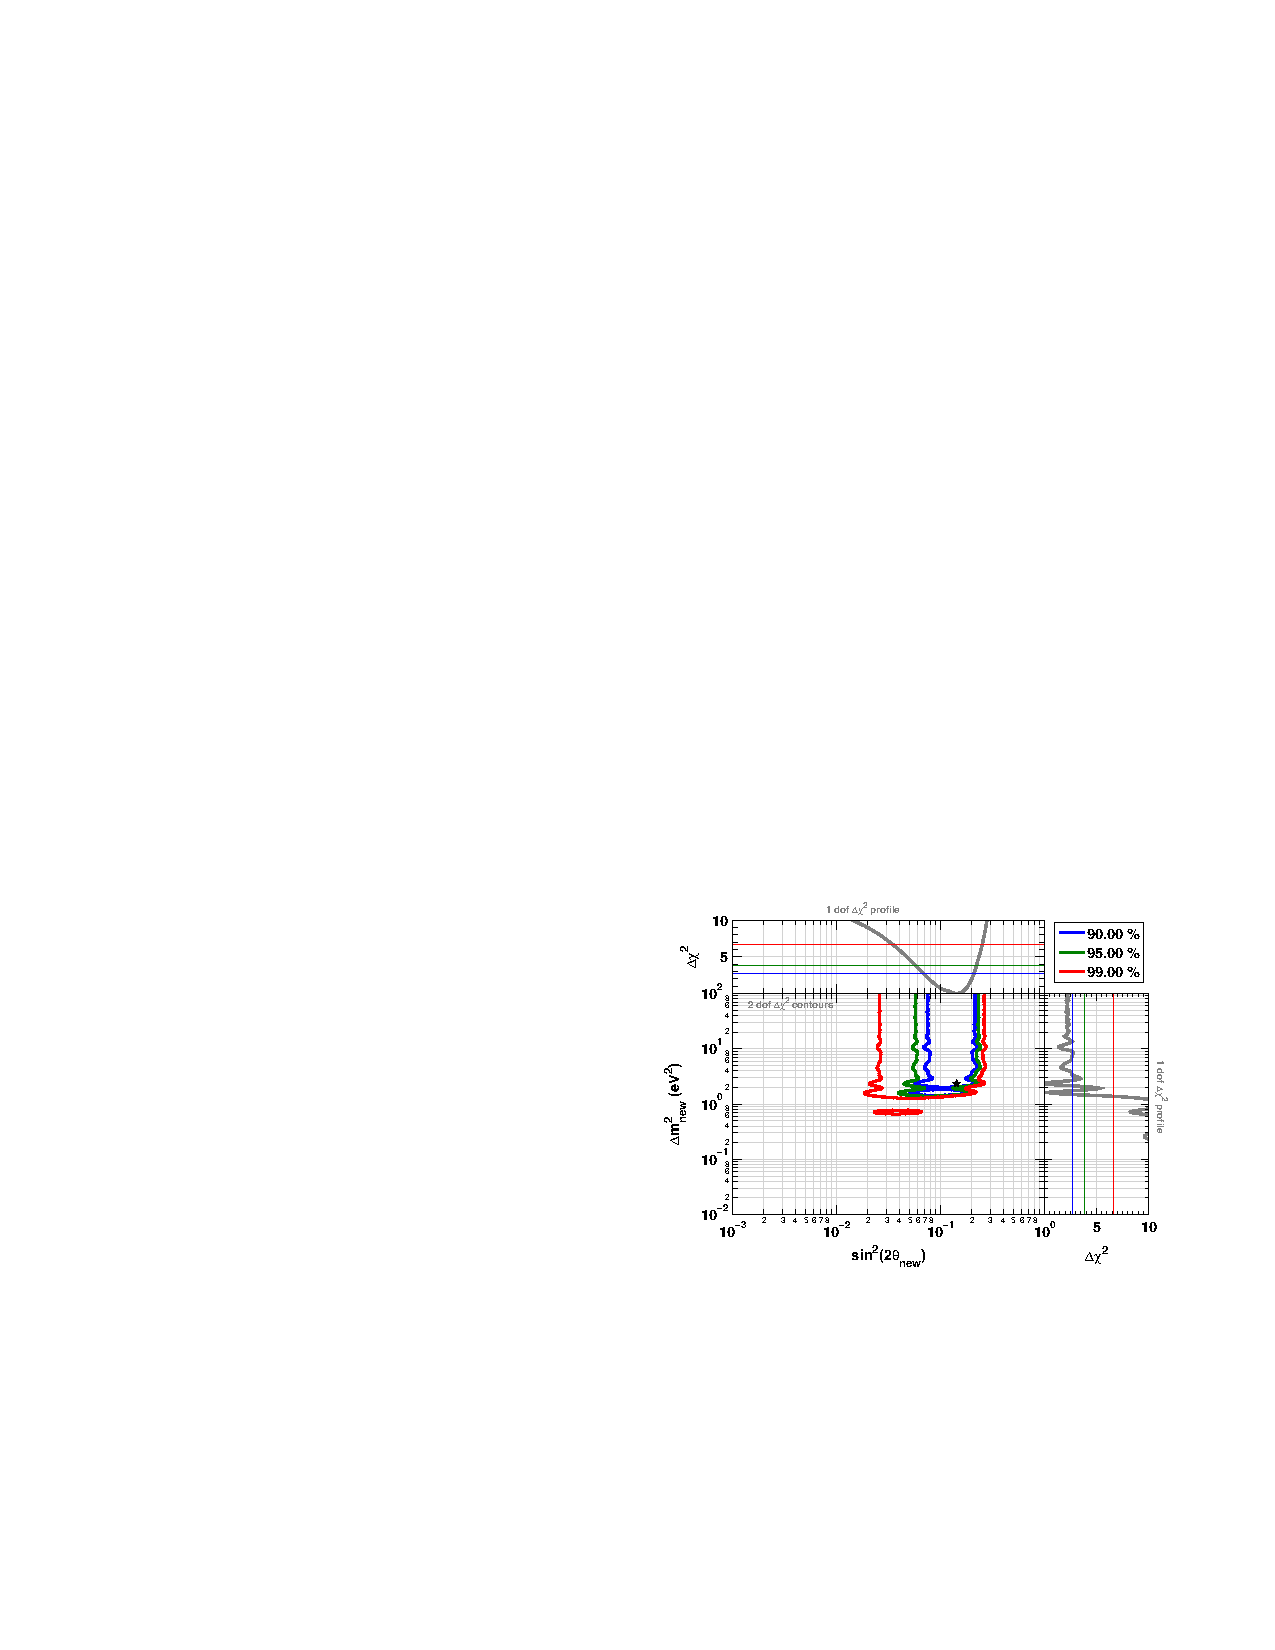
\includegraphics[width=0.8\textwidth]{Figures/RAA3plus1.pdf}
    \caption[The allowed region for the parameters of sterile oscillation]{The allowed region for the parameters of sterile neutrino oscillation as a result of the flux deficit observed in RAA~\cite{bib:RAA}. The best fit point suggests a $\sin_{14}^22\theta = 0.14\pm0.08$ and $|\Delta m^2| > 1.5$~eV$^2$ (95\% C.L.) of a 3+1 left hand neutrino and sterile neutrino mixing.}
    \label{fig:RAA}
\end{figure}

    Independent of the flux deviation, the medium baseline experiments Daya Bay~\cite{bib:DYBSpectrum}, Double CHOOZ~\cite{bib:DBChooz}, and RENO~\cite{bib:RENO}, also measured reactor neutrino spectra that disagree	 with the Huber and Mueller models, as shown in Figure~\ref{fig:DYBSpectrum}.
    An 8\% to 10\% excess is observed in the 4~MeV to 6~MeV region of IBD positron energy, equivalent to 5~MeV to 7~MeV reactor neutrino energy.
    With high statistical significance, the spectral deficit observed hints at errors in the nuclear database used to calculate the expected spectral shape.
    Additionally, the isotopic contribution to the flux and spectrum anomalies is unclear due to the mixture and evolution of the fission isotopes in the LEU reactors utilized by these experiments.
 \begin{figure}[h!]
    \centering
    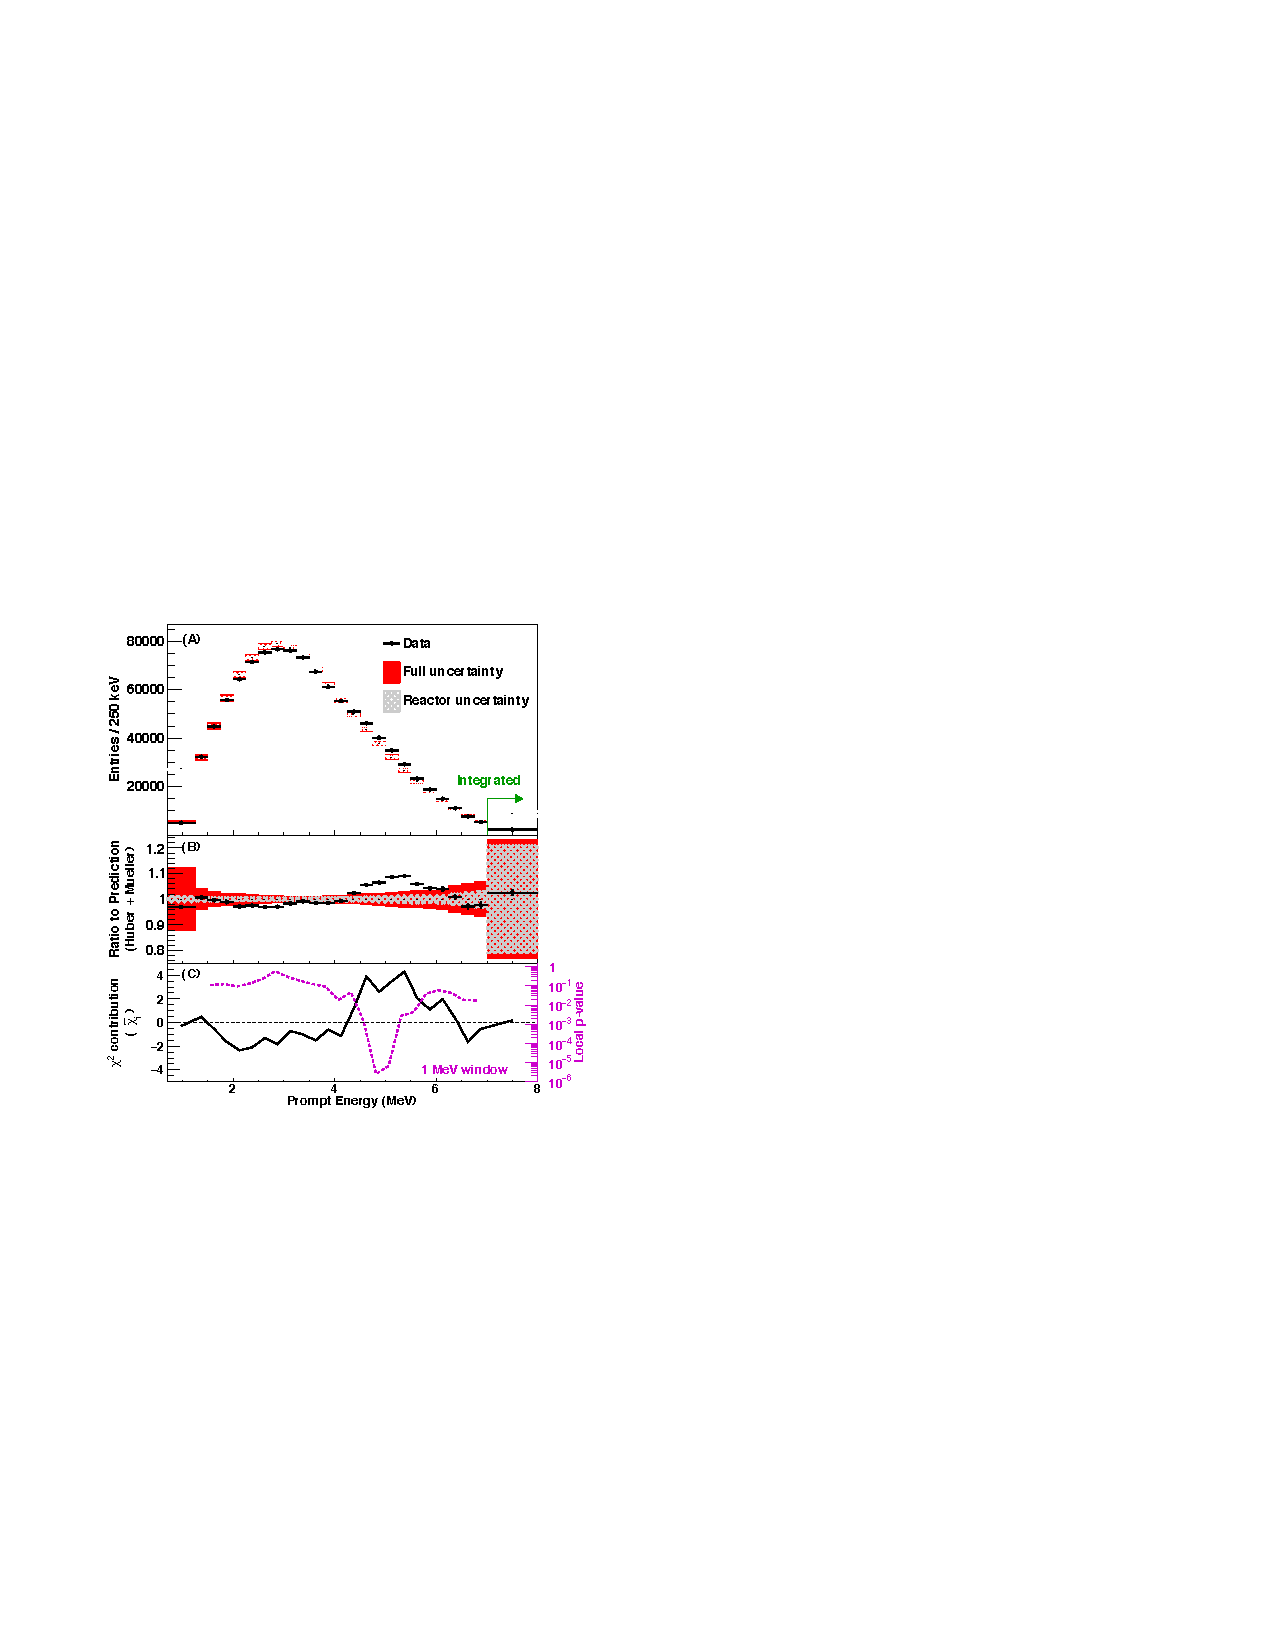
\includegraphics[width=0.8\textwidth]{Figures/DYBSpectrum.pdf}
    \caption[Daya Bay IBD positron energy spectrum]{The IBD positron energy spectrum measured by Daya Bay experiment.
    The spectrum is the sum of IBD positron spectrum from four fission isotopes, which indicate an excess at 4~MeV to 6~MeV compared to the Huber+Mueller model with 2.9~$\sigma$ discrepancy.}
    \label{fig:DYBSpectrum}
    
\end{figure} 
    
\Section{Resolution of the RAA}

    Further studies include introducing forbidden transitions in $\beta$-decay branch spectra~\cite{bib:hayes}, and \textit{ab initio} spectrum prediction with different nuclear databases~\cite{bib:dwyer}.
    These studies suggest larger systematic uncertainties than claimed in the Huber and Mueller model because of the lack of forbidden branch knowledge and errors in nuclear databases.
    Phenomenological studies~\cite{bib:giunti2019} based on historical reactor experiments were also made to resolve the RAA by comparing the neutrino flux of reactors with various fission fractions.
    The global fit of isotopic contributions to the flux deficit hint at $^{235}$U being the main contributor to the flux anomaly. 
    
    Multiple reactor neutrino measurements have been made to resolve the isotopic contribution of the flux and spectrum anomalies.
    Daya Bay and RENO experiments measured the reactor neutrino flux and spectrum evolution with fission fraction in their reactors~\cite{bib:DYBEvo, bib:RENOevolution}. 
    These measurements indirectly tested $^{235}$U and $^{239}$Pu's contribution to the reactor neutrino flux and spectrum deficit.
    In these fuel evolution measurements, the reactor neutrino flux and spectrum's dependence on fission isotope is observed.
    The evolution of the spectrum weakly hints at a correlation between the $^{235}$U-$^{239}$Pu transition and the local excess of the IBD spectrum.

    The lack of definitive resolution to the RAA the necessitates a direct measurement of the reactor neutrino flux and spectrum from a single fission isotope, particularly $^{235}$U.
    A very short baseline, $^{235}$U-only reactor neutrino experiment is preferred to measure the flux and spectrum of \nuebar from the single fission isotope, as well as to simultaneously and independently probe possible eV-scale sterile neutrino oscillations.
